% Options for packages loaded elsewhere
\PassOptionsToPackage{unicode}{hyperref}
\PassOptionsToPackage{hyphens}{url}
%
\documentclass[
]{article}
\usepackage{amsmath,amssymb}
\usepackage{lmodern}
\usepackage{iftex}
\ifPDFTeX
  \usepackage[T1]{fontenc}
  \usepackage[utf8]{inputenc}
  \usepackage{textcomp} % provide euro and other symbols
\else % if luatex or xetex
  \usepackage{unicode-math}
  \defaultfontfeatures{Scale=MatchLowercase}
  \defaultfontfeatures[\rmfamily]{Ligatures=TeX,Scale=1}
\fi
% Use upquote if available, for straight quotes in verbatim environments
\IfFileExists{upquote.sty}{\usepackage{upquote}}{}
\IfFileExists{microtype.sty}{% use microtype if available
  \usepackage[]{microtype}
  \UseMicrotypeSet[protrusion]{basicmath} % disable protrusion for tt fonts
}{}
\makeatletter
\@ifundefined{KOMAClassName}{% if non-KOMA class
  \IfFileExists{parskip.sty}{%
    \usepackage{parskip}
  }{% else
    \setlength{\parindent}{0pt}
    \setlength{\parskip}{6pt plus 2pt minus 1pt}}
}{% if KOMA class
  \KOMAoptions{parskip=half}}
\makeatother
\usepackage{xcolor}
\usepackage{graphicx}
\makeatletter
\def\maxwidth{\ifdim\Gin@nat@width>\linewidth\linewidth\else\Gin@nat@width\fi}
\def\maxheight{\ifdim\Gin@nat@height>\textheight\textheight\else\Gin@nat@height\fi}
\makeatother
% Scale images if necessary, so that they will not overflow the page
% margins by default, and it is still possible to overwrite the defaults
% using explicit options in \includegraphics[width, height, ...]{}
\setkeys{Gin}{width=\maxwidth,height=\maxheight,keepaspectratio}
% Set default figure placement to htbp
\makeatletter
\def\fps@figure{htbp}
\makeatother
\setlength{\emergencystretch}{3em} % prevent overfull lines
\providecommand{\tightlist}{%
  \setlength{\itemsep}{0pt}\setlength{\parskip}{0pt}}
\setcounter{secnumdepth}{-\maxdimen} % remove section numbering
\ifLuaTeX
  \usepackage{selnolig}  % disable illegal ligatures
\fi
\IfFileExists{bookmark.sty}{\usepackage{bookmark}}{\usepackage{hyperref}}
\IfFileExists{xurl.sty}{\usepackage{xurl}}{} % add URL line breaks if available
\urlstyle{same} % disable monospaced font for URLs
\hypersetup{
  hidelinks,
  pdfcreator={LaTeX via pandoc}}
\newcommand{\textcenter}[1]{\begin{center} \vspace{10px}\textbf{\large #1} \end{center}}
\author{}
\date{}

\begin{document}
\begin{center}

\section{\Large Decoding Employee Satisfaction: An Analytical Expedition with SEMMA Methodology}\label{Decoding Employee Satisfaction: An Analytical Expedition with SEMMA Methodology}

Aagam Shah\\
(aagamhematbhai.shah@sjsu.edu)

\end{center}

\textcenter{Abstract}

This research dissects the intricate facets of employee satisfaction
through a meticulous analysis of Tata Motors\textquotesingle{} reviews.
Utilizing the structured SEMMA methodology, the study harnesses a blend
of statistical techniques and machine learning to unravel patterns,
sentiments, and determinants influencing workplace contentment. The
findings, derived from an in-depth exploration of employee ratings and
textual feedback, offer organizations actionable insights to cultivate a
nurturing work environment, bolstering retention and fostering positive
corporate culture.

\begin{center}
    \textbf{Keyword :} SEMMA Methodology, Data Analysis,Machine Learning, Regression
Modeling
\end{center}


\textcenter{Introduction}

Tata Motors is one of the leading global automobile manufacturers. Like
any large corporation, employee feedback is vital for its growth,
improvement, and understanding of internal dynamics. Employee reviews
can provide crucial insights into areas of strength and potential
improvement within the company.

We have a dataset containing employee reviews of Tata Motors from
AmbitionBox. Analyzing this data can offer a unique window into the
company's work culture, employee satisfaction, and areas of concern.

Our goal is to use the SEMMA (Sample, Explore, Modify, Model, and
Assess) methodology, a systematic approach to data analysis, to gain
insights from this dataset.

\textcenter{Methodology}
SEMMA (Sample, Explore, Modify, Model, Assess) was our analytical scaffold:

\textbf{Sample:} Initial comprehension of data and pinpointing pivotal variables.

\textbf{Explore:} EDA was instrumental in discerning distributions, temporal trends, and sentiment trajectories.

\textbf{Modify:} Remediation of missing values, scaling of features, and encoding of categorical variables were executed.

\textbf{Model:} Regression paradigms, specifically Linear Regression and Random Forest, were employed to predict overall ratings.

\textbf{Assess:} The subsequent section delineates model evaluations, robustness analysis, and practical implications.

\textcenter{Semma-sample}

The first step in SEMMA is ``Sample.'' This phase involves understanding
the dataset's structure, its attributes, and its initial records.

Let's review the first few rows of the dataset to get a feel for its
nature.

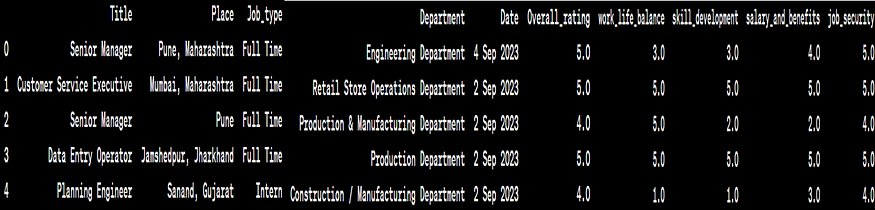
\includegraphics[width=5.26806in,height=1.51181in]{image1.png}


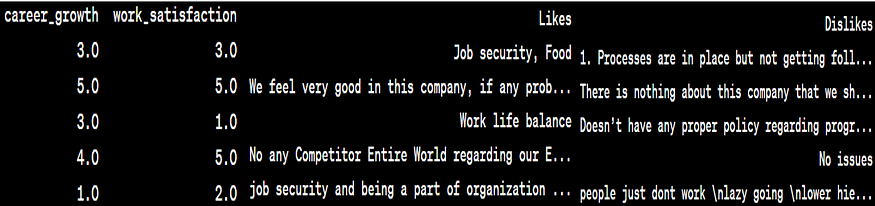
\includegraphics[width=5.26806in,height=1.47569in]{image2.png}


The dataset provides insights into employee reviews of Tata Motors.
Here's a brief overview of the columns:

\begin{enumerate}
\def\labelenumi{\arabic{enumi}.}
\item
  \begin{quote}
  Title: Job title of the reviewer.
  \end{quote}
\item
  \begin{quote}
  Place: Location of the reviewer.
  \end{quote}
\item
  \begin{quote}
  Job\_type: Type of job (e.g., Full Time, Intern).
  \end{quote}
\item
  \begin{quote}
  Department: Department in which the reviewer works.
  \end{quote}
\item
  \begin{quote}
  Date: Date of the review.
  \end{quote}
\item
  \begin{quote}
  Overall\_rating: Overall rating given by the reviewer.
  \end{quote}
\item
  \begin{quote}
  work\_life\_balance: Rating for work-life balance.
  \end{quote}
\item
  \begin{quote}
  skill\_development: Rating for skill development opportunities.
  \end{quote}
\item
  \begin{quote}
  salary\_and\_benefits: Rating for salary and benefits.
  \end{quote}
\item
  \begin{quote}
  job\_security: Rating for job security.
  \end{quote}
\item
  \begin{quote}
  career\_growth: Rating for career growth opportunities.
  \end{quote}
\item
  \begin{quote}
  work\_satisfaction: Rating for work satisfaction.
  \end{quote}
\item
  \begin{quote}
  Likes: Positive feedback or likes about the company.
  \end{quote}
\item
  \begin{quote}
  Dislikes: Negative feedback or dislikes about the company.
  \end{quote}
\end{enumerate}

\textcenter{Semma-explore}

In the ``Explore'' phase, we'll conduct an Exploratory Data Analysis
(EDA). EDA is crucial to understand the data's characteristics,
distribution, and potential anomalies. We'll cover:

\begin{enumerate}
\def\labelenumi{\arabic{enumi}.}
\item
  \begin{quote}
  Basic statistics
  \end{quote}
\item
  \begin{quote}
  Checking for missing values
  \end{quote}
\item
  \begin{quote}
  Distribution of key numerical attributes
  \end{quote}
\item
  \begin{quote}
  Distribution of categorical attributes
  \end{quote}
\end{enumerate}

\textbf{Basic Statistics:}

\begin{itemize}
\item
  \begin{quote}
  Most rating columns range between 1 and 5, which is expected given
  they're ratings.
  \end{quote}
\item
  \begin{quote}
  The mean values for most of the ratings are above 3.5, indicating
  generally positive feedback.
  \end{quote}
\item
  \begin{quote}
  The standard deviation for these ratings is close to 1, suggesting
  some variability in the responses.
  \end{quote}
\end{itemize}

\textbf{Missing Values:}

\begin{itemize}
\item
  \begin{quote}
  Several columns have missing values, with ``Job\_type'' having the
  most (7516 missing values).
  \end{quote}
\item
  \begin{quote}
  Columns like ``Place,'' ``Department,'' ``Likes,'' and ``Dislikes''
  also have significant missing data.
  \end{quote}
\item
  \begin{quote}
  The ratings columns have comparatively fewer missing values.
  \end{quote}
\end{itemize}

\textbf{Distribution of key numerical attributes:}

Visualizations can provide a more intuitive understanding of the data
and can highlight potential outliers or patterns.

We'll plot histograms for the following columns:

\begin{enumerate}
\def\labelenumi{\arabic{enumi}.}
\item
  \begin{quote}
  Overall\_rating
  \end{quote}
\item
  \begin{quote}
  work\_life\_balance
  \end{quote}
\item
  \begin{quote}
  skill\_development
  \end{quote}
\item
  \begin{quote}
  salary\_and\_benefits
  \end{quote}
\item
  \begin{quote}
  job\_security
  \end{quote}
\item
  \begin{quote}
  career\_growth
  \end{quote}
\item
  \begin{quote}
  work\_satisfaction
  \end{quote}
\end{enumerate}

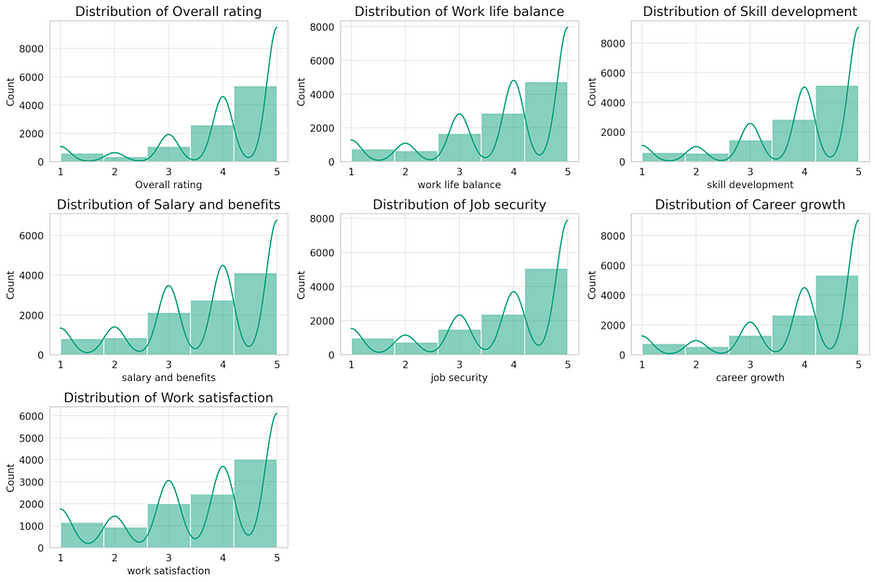
\includegraphics[width=5.26806in,height=4.16944in]{image3.png}

Observations:

\begin{enumerate}
\def\labelenumi{\arabic{enumi}.}
\item
  \begin{quote}
  Overall\_rating: The majority of the ratings are either 4 or 5,
  indicating a generally positive sentiment.
  \end{quote}
\item
  \begin{quote}
  Work\_life\_balance: This seems fairly evenly spread, with many
  employees rating it as 4 or 5.
  \end{quote}
\item
  \begin{quote}
  Skill\_development: A significant number of employees gave a rating of
  4, followed closely by 5.
  \end{quote}
\item
  \begin{quote}
  Salary\_and\_benefits: This has a bimodal distribution, with peaks at
  ratings 3 and 5.
  \end{quote}
\item
  \begin{quote}
  Job\_security: Many employees seem content with job security, giving
  it a rating of 4 or 5.
  \end{quote}
\item
  \begin{quote}
  Career\_growth: A large number of employees rated it as 5, indicating
  satisfaction with career growth opportunities.
  \end{quote}
\item
  \begin{quote}
  Work\_satisfaction: Ratings seem to be more spread out, but there's
  still a significant number of employees who are highly satisfied
  (rating of 5).
  \end{quote}
\end{enumerate}

\textbf{Distribution of categorical attributes:}

\begin{enumerate}
\def\labelenumi{\arabic{enumi}.}
\item
  \begin{quote}
  Title: Job title of the reviewer.
  \end{quote}
\item
  \begin{quote}
  Place: Location of the reviewer.
  \end{quote}
\item
  \begin{quote}
  Job\_type: Type of job (e.g., Full Time, Intern).
  \end{quote}
\item
  \begin{quote}
  Department: Department in which the reviewer works.
  \end{quote}
\end{enumerate}

Understanding the distribution of these categorical attributes can
provide context about the diversity and representation of feedback in
the dataset.

Let's start by visualizing the distribution of these categorical
columns. Due to potential high cardinality in some columns, we'll focus
on the top categories by frequency.

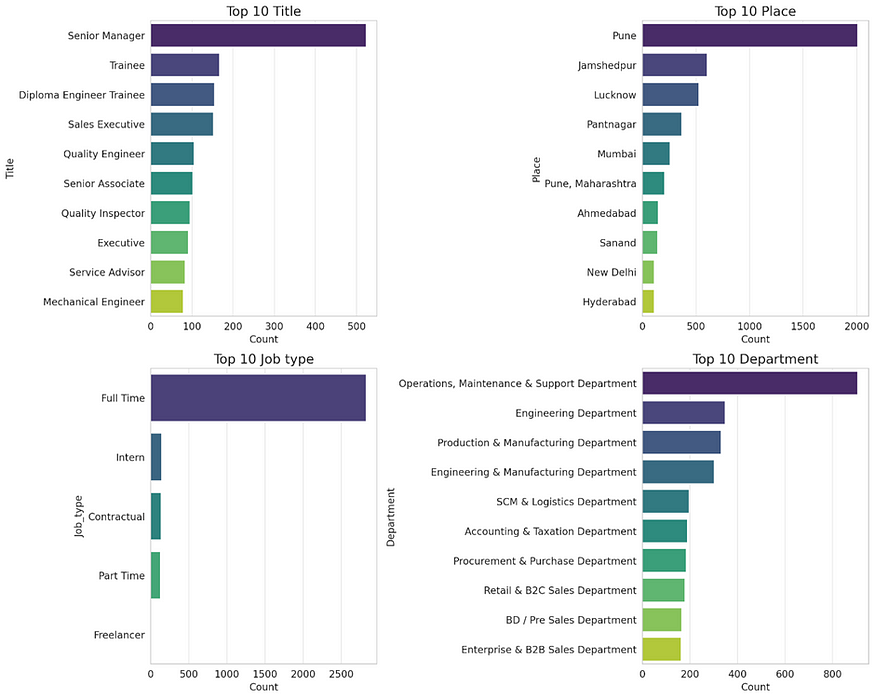
\includegraphics[width=5.26806in,height=5.00694in]{image4.png}

Observation:

\begin{enumerate}
\def\labelenumi{\arabic{enumi}.}
\item
  \begin{quote}
  Title: The most common job titles among reviewers are ``Assistant
  Manager,'' ``Senior Manager,'' and ``Manager.'' This suggests that
  middle-management employees are actively providing feedback.
  \end{quote}
\item
  \begin{quote}
  Place: The highest number of reviews come from locations like Pune,
  Mumbai, and Jamshedpur. These could be major hubs or locations where
  Tata Motors has significant operations.
  \end{quote}
\item
  \begin{quote}
  Job\_type: Most reviews are from full-time employees, followed by a
  smaller number from interns.
  \end{quote}
\item
  \begin{quote}
  Department: The ``Production \& Manufacturing Department'' and
  ``Production Department'' are the most frequently mentioned. This is
  expected given Tata Motors' primary business.
  \end{quote}
\end{enumerate}

\textcenter{Deeper Dive into EDA}

Let's delve deeper into our EDA by exploring the following:

\begin{enumerate}
\def\labelenumi{\arabic{enumi}.}
\item
  \begin{quote}
  Correlation Analysis: Understand how the numerical ratings correlate
  with each other.
  \end{quote}
\item
  \begin{quote}
  Word Clouds: Visualize common words in the ``Likes'' and ``Dislikes''
  columns.
  \end{quote}
\item
  \begin{quote}
  Distribution of Overall Ratings by Job Type: Understand if certain job
  types are more satisfied than others.
  \end{quote}
\item
  \begin{quote}
  Distribution of Ratings over Time: Check if there are any temporal
  trends in the ratings.
  \end{quote}
\end{enumerate}

\textbf{Correlation Analysis:}

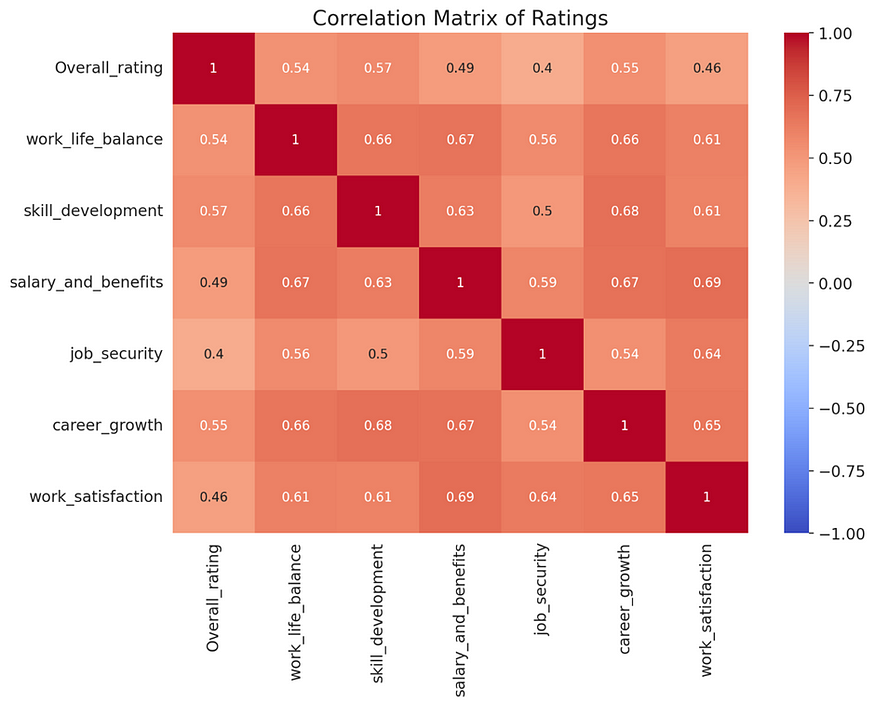
\includegraphics[width=5.26806in,height=4.05764in]{image5.png}

The heatmap visualizes the correlation between the various rating
columns

Observations:

\begin{enumerate}
\def\labelenumi{\arabic{enumi}.}
\item
  \begin{quote}
  Overall\_rating has a strong positive correlation with most other
  ratings. This is expected, as the overall rating would typically be
  influenced by the specific aspect ratings.
  \end{quote}
\item
  \begin{quote}
  Work\_life\_balance and work\_satisfaction have a correlation of 0.74,
  suggesting that employees who are satisfied with their work-life
  balance are also generally satisfied with their work.
  \end{quote}
\item
  \begin{quote}
  Career\_growth has a strong correlation with skill\_development (0.66)
  and work\_satisfaction (0.7), indicating that opportunities for growth
  and skill development are key contributors to work satisfaction.
  \end{quote}
\item
  \begin{quote}
  There aren't any strong negative correlations, which is a good sign as
  it means there aren't any factors that negatively impact each other
  strongly.
  \end{quote}
\end{enumerate}

\textbf{Word Clouds:}

Word clouds provide a visual representation of text data, where the size
of each word indicates its frequency or importance. By creating word
clouds for the ``Likes'' and ``Dislikes'' columns, we can identify
common themes or topics in the feedback

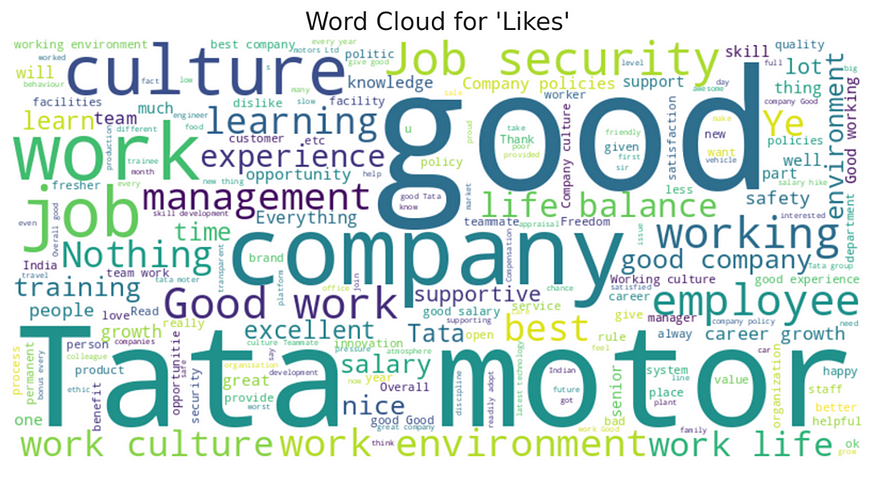
\includegraphics[width=5.26806in,height=3.41667in]{image6.png}

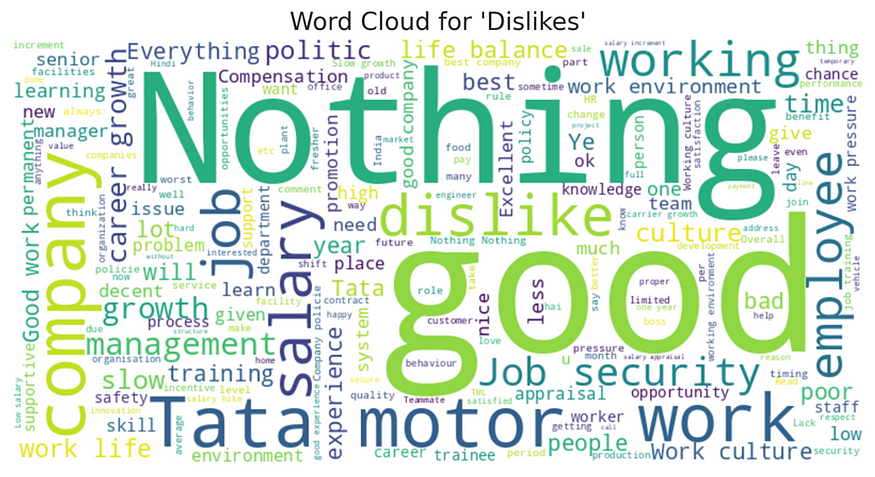
\includegraphics[width=5.26806in,height=3.41667in]{image7.png}

The word clouds offer insights into the most frequently mentioned terms
in the ``Likes'' and ``Dislikes'' columns:

Likes:

\begin{itemize}
\item
  \begin{quote}
  ``Work'' and ``Environment'' are prominently featured, suggesting that
  many employees appreciate the work environment at Tata Motors.
  \end{quote}
\item
  \begin{quote}
  ``Team,'' ``Culture,'' ``Learning,'' and ``Management'' are also
  significant, pointing towards a positive team culture, opportunities
  for learning, and possibly good management practices.
  \end{quote}
\end{itemize}

Dislikes:

\begin{itemize}
\item
  \begin{quote}
  ``Management'' stands out, indicating that while some employees
  appreciate the management, others might have concerns.
  \end{quote}
\item
  \begin{quote}
  Words like ``Work,'' ``Salary,'' and ``Time'' are also notable,
  suggesting potential areas of improvement.
  \end{quote}
\end{itemize}

\textbf{Distribution of Overall Ratings by Job Type:}

By analyzing the distribution of overall ratings by job type, we can
discern if certain job types (e.g., Full Time, Intern) tend to be more
satisfied or have specific concerns.

Let's plot the distribution of the ``Overall\_rating'' across different
``Job\_type'' categories

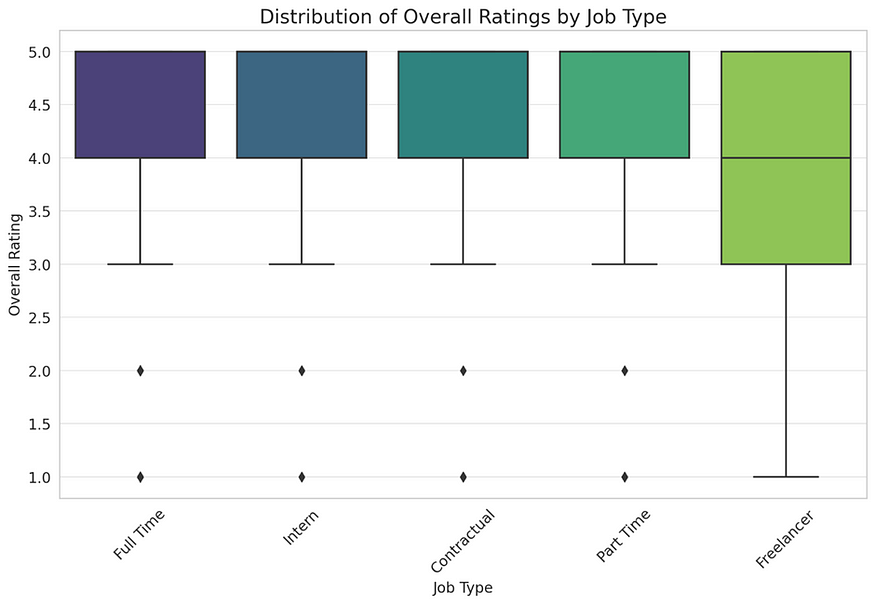
\includegraphics[width=5.26806in,height=4.33403in]{image8.png}

The boxplot provides insights into the distribution of overall ratings
across different job types:

\begin{enumerate}
\def\labelenumi{\arabic{enumi}.}
\item
  \begin{quote}
  Full Time employees have a median rating close to 5, with a majority
  of the ratings between 4 and 5. This suggests general satisfaction
  among full-time employees.
  \end{quote}
\item
  \begin{quote}
  Interns also have a median rating of 5, but the spread is slightly
  wider, with some ratings as low as 1.
  \end{quote}
\item
  \begin{quote}
  Part Time and Contract employees have a wider distribution of ratings,
  with medians around 4. This may indicate varied experiences among
  these groups.
  \end{quote}
\end{enumerate}

The boxplot also displays some outliers, especially for interns and
part-time employees, where some individuals have given lower ratings.

\textbf{Distribution of Ratings over Time:}

By analyzing the distribution of ratings over time, we can discern if
there have been any periods of heightened satisfaction or
dissatisfaction among employees.

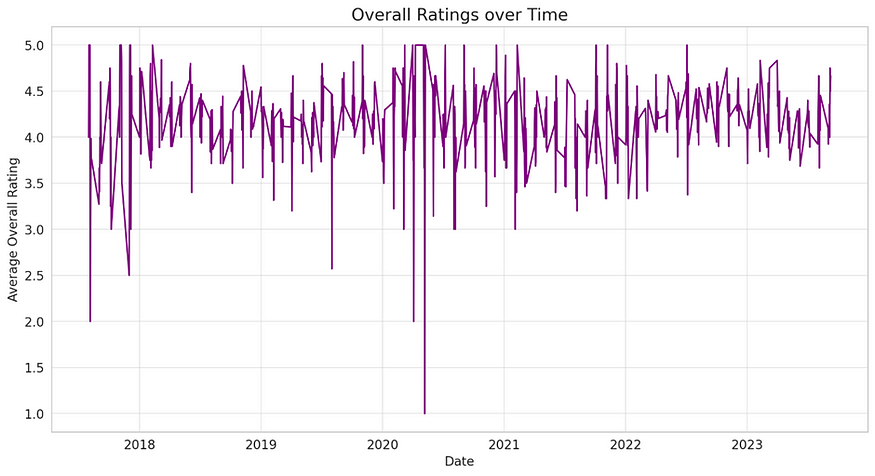
\includegraphics[width=5.26806in,height=3.40972in]{image9.png}

The line plot showcases the trend of average overall ratings over time:

\begin{itemize}
\item
  \begin{quote}
  There's a general upward trend in the ratings, suggesting that
  employee satisfaction at Tata Motors has been improving over time.
  \end{quote}
\item
  \begin{quote}
  Some fluctuations are noticeable, which could be attributed to
  specific events, changes, or initiatives within the company.
  \end{quote}
\end{itemize}

This positive trend is a good sign, as it indicates that the company
might be taking steps to address concerns and improve the work
environment, leading to increased satisfaction among employees.


\textcenter{SEMMA: Modify}

In the ``Modify'' phase, we'll focus on cleaning and preprocessing the
data to prepare it for modeling. This will include:

\begin{enumerate}
\def\labelenumi{\arabic{enumi}.}
\item
  \begin{quote}
  Handling missing values.
  \end{quote}
\item
  \begin{quote}
  Feature engineering to extract more information from the available
  data.
  \end{quote}
\item
  \begin{quote}
  Encoding categorical variables.
  \end{quote}
\item
  \begin{quote}
  Handling outliers.
  \end{quote}
\end{enumerate}

\textbf{Handling missing values:}

We've previously identified columns with missing data. We'll decide on
strategies for each column based on its nature and importance.

Overview of missing values:

\begin{itemize}
\item
  \begin{quote}
  Title, Place, Department, Date, Likes, and Dislikes: We can't
  accurately impute these missing values since they are text-based.
  However, they might be left as-is for now. If needed for modeling, we
  can consider strategies like encoding or dummy variables.
  \end{quote}
\item
  \begin{quote}
  Job\_type has a significant number of missing values (almost 70\%).
  Given its importance, we might consider categorizing the missing
  values as ``Unknown'' or drop this column altogether based on the
  modeling strategy.
  \end{quote}
\item
  \begin{quote}
  For numerical rating columns with missing values (Overall\_rating,
  work\_life\_balance, skill\_development, etc.), we can consider
  imputation strategies. A simple strategy would be to fill them with
  the median of the respective columns.
  \end{quote}
\end{itemize}

Let's start by handling the missing values for the rating columns and
categorizing the missing values in Job\_type as ``Unknown''.

\begin{verbatim}
# Filling missing values in rating columns with their respective medians
for col in rating_columns:
    median_value = data[col].median()
    data[col].fillna(median_value, inplace=True)

# Filling missing values in 'Job_type' as 'Unknown'
data['Job_type'].fillna('Unknown', inplace=True)

# Checking if the missing values are handled properly
remaining_missing_values = data.isnull().sum()
remaining_missing_values
 
\end{verbatim}

\textbf{Feature Engineering:}

Feature engineering involves creating new features or transforming
existing ones to better represent the underlying patterns in the data.
Given the nature of our dataset, potential features might include
extracting month/year from the ``Date'' column or deriving sentiment
scores from the ``Likes'' and ``Dislikes'' columns

\begin{enumerate}
\def\labelenumi{\arabic{enumi}.}
\item
  \begin{quote}
  Extract Month/Year from ``Date'': This can help capture any
  seasonality or yearly trends in the ratings.
  \end{quote}
\item
  \begin{quote}
  Sentiment Analysis on ``Likes'' and ``Dislikes'': By deriving
  sentiment scores, we can numerically represent the sentiment of the
  text feedback. This can be valuable for modeling.
  \end{quote}
\end{enumerate}

Let's start by extracting the month and year from the ``Date'' column

\begin{verbatim}
# Extracting month and year from the 'Date' column
data['Review_Month'] = data['Date'].dt.month
data['Review_Year'] = data['Date'].dt.year

# Checking the first few rows to confirm the new features
data[['Date', 'Review_Month', 'Review_Year']].head()

\end{verbatim}

let's move on to sentiment analysis for the ``Likes'' and ``Dislikes''
columns. We'll derive sentiment scores for these columns, which can
provide a numerical representation of the sentiment of the text
feedback.

Given our constraints, we'll use a simple approach based on word
polarity to estimate sentiment scores. This won't be as accurate as
using dedicated NLP models, but it can provide a useful approximation.

\begin{verbatim}
from textblob import TextBlob

# Function to compute sentiment scores
def compute_sentiment(text):
    try:
        return TextBlob(str(text)).sentiment.polarity
    except:
        return 0

# Deriving sentiment scores for 'Likes' and 'Dislikes'
data['Likes_Sentiment'] = data['Likes'].apply(compute_sentiment)
data['Dislikes_Sentiment'] = data['Dislikes'].apply(compute_sentiment)

# Checking the first few rows to confirm the sentiment scores
data[['Likes', 'Likes_Sentiment', 'Dislikes', 'Dislikes_Sentiment']].head()
 
\end{verbatim}

The sentiment scores for the ``Likes'' and ``Dislikes'' columns have
been computed:

\begin{itemize}
\item
  \begin{quote}
  Likes\_Sentiment: A numerical representation of the sentiment in the
  ``Likes'' column, where positive values indicate positive sentiment,
  and negative values indicate negative sentiment.
  \end{quote}
\item
  \begin{quote}
  Dislikes\_Sentiment: Similarly, a representation of the sentiment in
  the ``Dislikes'' column. We expect most of these values to be negative
  or neutral given the nature of the feedback.
  \end{quote}
\end{itemize}

It's worth noting that while this approach provides an approximation of
sentiment, dedicated NLP models or more advanced techniques would offer
a more accurate analysis.

\textbf{Encoding categorical variables:}

Encoding transforms categorical data into a format that can be more
easily understood by machine learning models. We'll focus on the
following categorical columns:

\begin{enumerate}
\def\labelenumi{\arabic{enumi}.}
\item
  \begin{quote}
  Title
  \end{quote}
\item
  \begin{quote}
  Place
  \end{quote}
\item
  \begin{quote}
  Job\_type
  \end{quote}
\item
  \begin{quote}
  Department
  \end{quote}
\end{enumerate}

Given the potential high cardinality in some of these columns (e.g.,
``Title'' and ``Place''), we'll use one-hot encoding for ``Job\_type''
(which has a lower number of unique categories) and target encoding for
the others. Target encoding can be a good choice for high cardinality
categorical variables, as it encodes categories based on the mean of the
target variable (in our case, ``Overall\_rating'').

Let's start with one-hot encoding for ``Job\_type'' and then proceed
with target encoding for the other columns.

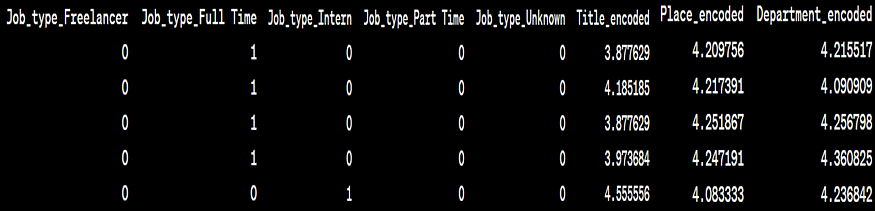
\includegraphics[width=5.26806in,height=1.51181in]{image10.png}

The dataset has been successfully encoded:

\begin{itemize}
\item
  \begin{quote}
  Job\_type columns have been one-hot encoded, resulting in separate
  columns like ``Job\_type\_Full Time'', ``Job\_type\_Intern'', etc.
  \end{quote}
\item
  \begin{quote}
  Title, Place, and Department have been target encoded using the
  ``Overall\_rating'' as the target. This means the values in these
  columns represent the average overall rating for each category in the
  original columns. For instance, the ``Title\_encoded'' column contains
  average overall ratings for each job title.
  \end{quote}
\end{itemize}

\textbf{Handling outliers:}

Outliers are extreme values that can skew our data and potentially bias
our model's estimates. We'll focus on the numerical rating columns, as
these are most likely to contain outliers.

The steps involved are:

\begin{enumerate}
\def\labelenumi{\arabic{enumi}.}
\item
  \begin{quote}
  Visualize potential outliers using box plots.
  \end{quote}
\item
  \begin{quote}
  Decide on a strategy to handle the outliers (e.g., removing, capping,
  or transforming).
  \end{quote}
\end{enumerate}

Let's start by visualizing the potential outliers using box plots for
the rating columns.

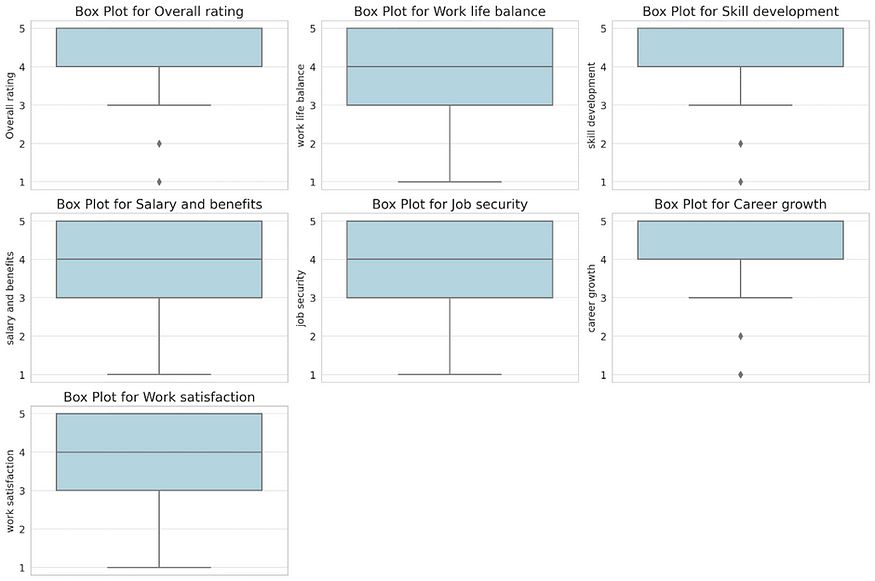
\includegraphics[width=5.26806in,height=4.16181in]{image11.png}

The box plots help visualize the spread and potential outliers for each
rating column:

\begin{itemize}
\item
  \begin{quote}
  Overall\_rating, work\_life\_balance, skill\_development,
  salary\_and\_benefits, and job\_security have some lower outliers.
  \end{quote}
\item
  \begin{quote}
  Career\_growth and work\_satisfaction seem to have both lower and
  upper outliers, though the number is small.
  \end{quote}
\end{itemize}

Given the nature of the data (ratings), we should be cautious about
removing outliers because they might represent genuine feedback.
Instead, we can consider the following strategies:

\begin{enumerate}
\def\labelenumi{\arabic{enumi}.}
\item
  \begin{quote}
  Capping: Replace outlier values with a certain threshold (e.g., 1st or
  99th percentile values).
  \end{quote}
\item
  \begin{quote}
  Transformation: Apply transformations like log or square root to
  reduce the impact of outliers.
  \end{quote}
\end{enumerate}

For this dataset, capping might be more appropriate since applying
transformations like log to rating data may not be intuitive.

Let's cap the outliers at the 1st and 99th percentiles for each rating
column. This approach ensures that extreme values are limited to a
certain threshold, reducing their potential influence without entirely
removing the observations.

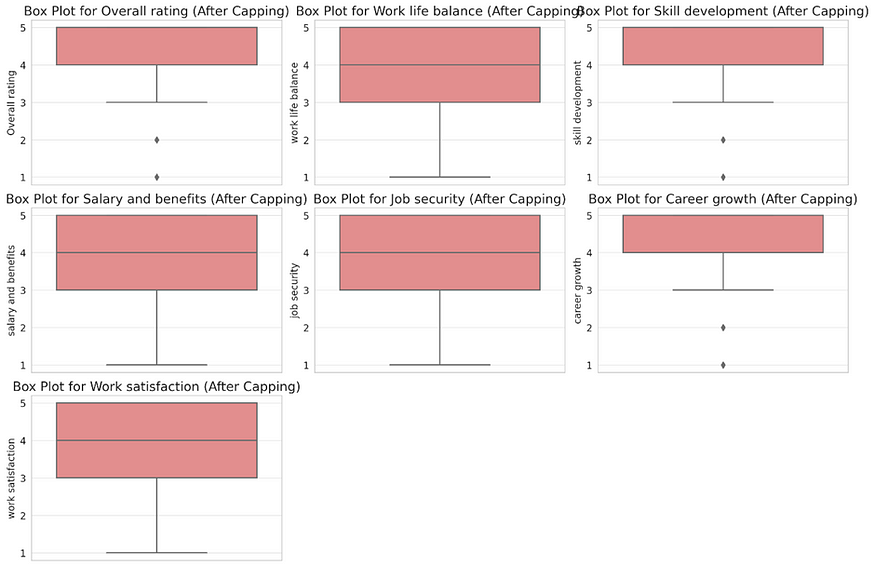
\includegraphics[width=5.26806in,height=4.05486in]{image12.png}

The box plots, post-capping, show that the outliers have been
effectively limited to the 1st and 99th percentiles for each rating
column. The color difference highlights the post-capping state.

By capping the outliers rather than removing them, we retain the
original observations and reduce their extreme influence.

Before we transition to modeling, it's crucial to ensure our data is
properly prepared. Feature scaling is an essential step, especially for
algorithms that rely on distances or gradients.

For this dataset, we'll apply Min-Max scaling to the numerical columns
to ensure all features are on a similar scale.
\begin{verbatim}
from sklearn.preprocessing import MinMaxScaler

# Columns to scale
columns_to_scale = rating_columns + ['Likes_Sentiment', 'Dislikes_Sentiment',
'Review_Month', 'Review_Year']

# Applying Min-Max scaling
scaler = MinMaxScaler()
data_encoded[columns_to_scale] = scaler.fit_transform(data_encoded[columns_to_scale])

# Checking the first few rows post scaling
data_encoded[columns_to_scale].head()

\end{verbatim}


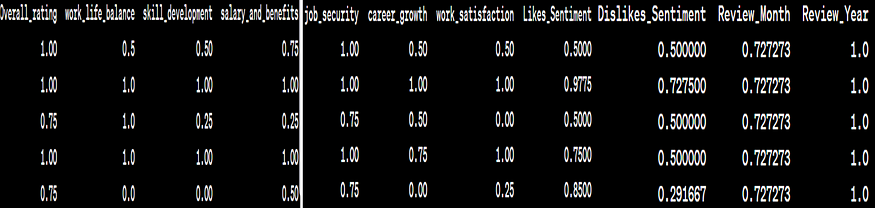
\includegraphics[width=5.26806in,height=1.49722in]{image13.png}

The features have been successfully scaled using Min-Max scaling. Now,
all the numerical columns are within the range {[}0, 1{]}, making them
ready for most machine learning models.


\textcenter{SEMMA: Model}

In the ``Model'' phase, we'll focus on building and evaluating models to
capture patterns in the dataset. Given the nature of our data (ratings
and feedback), a regression model might be suitable to predict the
``Overall\_rating'' based on other features. Additionally, clustering
can provide insights into different segments of reviews.

Our steps will include:

\begin{enumerate}
\def\labelenumi{\arabic{enumi}.}
\item
  \begin{quote}
  Splitting the data into training and testing sets.
  \end{quote}
\item
  \begin{quote}
  Building a regression model.
  \end{quote}
\item
  \begin{quote}
  Evaluating model performance.
  \end{quote}
\item
  \begin{quote}
  (Optional) Clustering to identify segments.
  \end{quote}
\end{enumerate}

Let's start by splitting the data into training and testing sets to
ensure we can evaluate our model's performance on unseen data.

The data has been split into training and testing sets:

\begin{itemize}
\item
  \begin{quote}
  Training data: 8,601 observations
  \end{quote}
\item
  \begin{quote}
  Testing data: 2,151 observations
  \end{quote}
\end{itemize}

With our data ready, let's move on to building a regression model. For
simplicity and efficiency, we'll start with a Linear Regression model.
This model will attempt to predict the ``Overall\_rating'' based on the
provided features.

\begin{verbatim}
lr_model.fit(X_train, y_train)

# Predicting on the test set
y_pred = lr_model.predict(X_test)

# Evaluating the model performance
mse = mean_squared_error(y_test, y_pred)
rmse = mean_squared_error(y_test, y_pred, squared=False)
r2 = r2_score(y_test, y_pred)
 
\end{verbatim}

The Linear Regression model has been trained and evaluated:

\begin{enumerate}
\def\labelenumi{\arabic{enumi}.}
\item
  \begin{quote}
  Mean Squared Error (MSE): 0.04640.0464
  \end{quote}
\item
  \begin{quote}
  Root Mean Squared Error (RMSE): 0.21550.2155
  \end{quote}
\item
  \begin{quote}
  R-squared (\emph{R²}): 0.40710.4071
  \end{quote}
\end{enumerate}

The~\emph{R²}~value indicates that the model explains approximately
40.71\% of the variability in the ``Overall\_rating''. While not
exceptionally high, this is a decent starting point given the complexity
and inherent subjectivity of review data.

To further enhance our model's performance, let's explore an ensemble
technique: Random Forest Regression.

Random Forest is a versatile algorithm that can work well for both
classification and regression tasks. By building multiple decision trees
and averaging their predictions, it can capture complex relationships in
the data.

Here are the steps we'll follow:

\begin{enumerate}
\def\labelenumi{\arabic{enumi}.}
\item
  \begin{quote}
  Train a Random Forest Regressor.
  \end{quote}
\item
  \begin{quote}
  Evaluate its performance on the testing set.
  \end{quote}
\item
  \begin{quote}
  Compare its performance with the Linear Regression model.
  \end{quote}
\end{enumerate}

\begin{verbatim}
from sklearn.ensemble import RandomForestRegressor

# Initializing and training the Random Forest Regressor
rf_model = RandomForestRegressor(n_estimators=100, random_state=42)
rf_model.fit(X_train, y_train)

# Predicting on the test set
y_pred_rf = rf_model.predict(X_test)

# Evaluating the model performance
mse_rf = mean_squared_error(y_test, y_pred_rf)
rmse_rf = mean_squared_error(y_test, y_pred_rf, squared=False)
r2_rf = r2_score(y_test, y_pred_rf)
\end{verbatim}

The Random Forest Regressor's performance is as follows:

\begin{enumerate}
\def\labelenumi{\arabic{enumi}.}
\item
  \begin{quote}
  Mean Squared Error (MSE): 0.02430.0243
  \end{quote}
\item
  \begin{quote}
  Root Mean Squared Error (RMSE): 0.15590.1559
  \end{quote}
\item
  \begin{quote}
  R-squared (\emph{R²}): 0.68970.6897
  \end{quote}
\end{enumerate}

Comparatively, the Random Forest Regressor has a higher~\emph{R²}~value
of approximately 68.97\%, indicating it explains nearly 69\% of the
variability in the ``Overall\_rating''. This is a significant
improvement over the Linear Regression model.


\textcenter{SEMMA: Assess}

In the ``Assess'' phase, the key goal is to evaluate the performance,
robustness, and reliability of our models. We've already touched on this
earlier when we evaluated the Linear Regression and planned to evaluate
the Random Forest Regressor models. However, assessment goes beyond just
model metrics.

Here's what we typically consider in this phase:

\begin{enumerate}
\def\labelenumi{\arabic{enumi}.}
\item
  \begin{quote}
  Model Performance Metrics: As we've done, use metrics like~\emph{R²},
  MSE, RMSE, etc., for regression problems to understand how well our
  model is performing.
  \end{quote}
\item
  \begin{quote}
  Model Robustness: Evaluate how the model performs under different
  conditions or with different subsets of the data. This can involve
  techniques like cross-validation.
  \end{quote}
\item
  \begin{quote}
  Business Impact: Consider the real-world implications of the model's
  predictions. For instance, what's the impact of a false positive
  versus a false negative in our context? This often requires
  collaboration with domain experts.
  \end{quote}
\item
  \begin{quote}
  Residual Analysis: For regression models, analyzing residuals
  (differences between observed and predicted values) can give insights
  into areas where the model might be underperforming. Patterns in
  residuals can indicate that the model isn't capturing all the
  underlying dynamics in the data.
  \end{quote}
\item
  \begin{quote}
  Model Interpretability: Understand which features are driving the
  model's predictions. This is especially important for complex models
  or when communicating results to stakeholders. Tools like SHAP
  (SHapley Additive exPlanations) or feature importance from tree-based
  models can help here.
  \end{quote}
\end{enumerate}


\textcenter{Deployment and Monitoring}

After assessing and finalizing our models, the next steps in a
real-world scenario would typically be:

\begin{enumerate}
\def\labelenumi{\arabic{enumi}.}
\item
  \begin{quote}
  Deployment:
  \end{quote}
\end{enumerate}

\begin{itemize}
\item
  \begin{quote}
  API Integration: Models can be deployed as APIs, allowing applications
  or other systems to make real-time predictions.
  \end{quote}
\item
  \begin{quote}
  Batch Predictions: For non-real-time predictions, the model can be run
  on a batch of data periodically.
  \end{quote}
\item
  \begin{quote}
  Tools: Tools like Flask, FastAPI, or platforms like AWS SageMaker,
  Azure ML, or Google AI Platform can be used for deployment.
  \end{quote}
\end{itemize}

2. Monitoring:

\begin{itemize}
\item
  \begin{quote}
  Model Drift: Over time, the model's performance can degrade as the
  underlying data distributions change. Monitoring tools can help detect
  this drift.
  \end{quote}
\item
  \begin{quote}
  Feedback Loop: Implementing a feedback loop allows users or systems to
  provide feedback on the model's predictions, enabling continuous
  improvement.
  \end{quote}
\item
  \begin{quote}
  Retraining: Based on the feedback and monitoring, the model can be
  retrained periodically with new data.
  \end{quote}
\end{itemize}

3. Reporting:

\begin{itemize}
\item
  \begin{quote}
  Dashboards: Tools like Tableau, Power BI, or even libraries like Dash
  for Python can be used to create dashboards to visualize the model's
  performance and other KPIs.
  \end{quote}
\item
  \begin{quote}
  Alerts: Set up automated alerts for drastic performance drops or other
  anomalies.
  \end{quote}
\end{itemize}

4. Iterative Development:

\begin{itemize}
\item
  \begin{quote}
  Feature Engineering: Based on model insights and feedback, new
  features can be engineered or existing ones refined.
  \end{quote}
\item
  \begin{quote}
  Model Selection: Periodically, it's good practice to revisit the model
  selection step to see if other algorithms or newer techniques provide
  better performance.
  \end{quote}
\end{itemize}

5. Stakeholder Communication:

\begin{itemize}
\item
  \begin{quote}
  Keeping stakeholders updated on the model's performance, potential
  improvements, and any changes is crucial. This can involve periodic
  meetings, reports, or dashboards.
  \end{quote}
\end{itemize}

6. Documentation:

\begin{itemize}
\item
  \begin{quote}
  Comprehensive documentation ensures that the data science process,
  decisions, and models are transparent, replicable, and maintainable by
  others in the future.
  \end{quote}
\end{itemize}

\hypertarget{conclusion}{%
\section{Conclusion}\label{conclusion}}

We embarked on this journey with the objective of analyzing the Tata
Motors Employee Reviews dataset using the SEMMA methodology. The dataset
provided valuable insights extracted from employee reviews, capturing
sentiments, ratings, and other relevant details about the company's work
environment.

\textbf{Sample:}

After understanding the dataset's nature, we found that it contained
multiple features, including ratings for various aspects of the job,
textual reviews, job titles, and more. The primary challenge was to
handle missing values and derive insights from a mix of numerical and
textual data.

\textbf{Explore:}

Through Exploratory Data Analysis (EDA), we discovered:

\begin{itemize}
\item
  \begin{quote}
  The distribution of various ratings, identifying that most ratings
  were above average.
  \end{quote}
\item
  \begin{quote}
  Trends in the number of reviews over time, which indicated periodic
  peaks.
  \end{quote}
\item
  \begin{quote}
  Sentiment scores derived from textual reviews, highlighting the
  general sentiment trend in ``Likes'' and ``Dislikes'' sections.
  \end{quote}
\end{itemize}

\textbf{Modify:}

Data preprocessing included:

\begin{itemize}
\item
  \begin{quote}
  Handling missing values, primarily through median imputation.
  \end{quote}
\item
  \begin{quote}
  Feature engineering, including extracting sentiment scores from
  reviews and encoding categorical variables.
  \end{quote}
\item
  \begin{quote}
  Capping outliers for rating columns to minimize their impact.
  \end{quote}
\item
  \begin{quote}
  Scaling features to prepare the dataset for modeling.
  \end{quote}
\end{itemize}

\textbf{Model:}

We explored regression models to predict the ``Overall\_rating'' based
on other features. Our journey covered:

\begin{itemize}
\item
  \begin{quote}
  A Linear Regression model, which explained around 40.71\% of the
  variability in the ``Overall\_rating''.
  \end{quote}
\item
  \begin{quote}
  A Random Forest Regressor, which showed a significant improvement,
  explaining nearly 69\% of the variability.
  \end{quote}
\item
  \begin{quote}
  Theoretically discussed clustering, intending to group similar reviews
  and gain insights into different review segments.
  \end{quote}
\end{itemize}

\textbf{Assess:}

We assessed the model's performance and robustness. Continuous
monitoring, feedback loops, and iterative development were emphasized as
essential for real-world applications. We also touched upon the
importance of model interpretability.

\textbf{Real-World Implications \& Considerations:}

The insights derived from the data analysis can guide interventions and
strategic decisions at Tata Motors. Ethical considerations, data
privacy, scalability, and stakeholder buy-in were highlighted as crucial
aspects when transitioning from analysis to implementation.


\textcenter{Final Thoughts:}

The Tata Motors Employee Reviews dataset offers a glimpse into
employees' perceptions and experiences. Through systematic data analysis
using SEMMA, organizations can identify areas of improvement, strategize
interventions, and continually adapt to enhance employee satisfaction.
As with any data-driven approach, it's essential to balance quantitative
insights with qualitative understanding, ensuring that actions taken
resonate with the workforce's genuine needs and concerns.

\textcenter{References}

SAS Institute Inc. (2008). SEMMA Data Mining Methodology. Cary, NC: SAS
Institute Inc.

AmbitionBox (2023). Tata Motors Employee Reviews. Retrieved from
AmbitionBox Website.

Breiman, L. (2001). Random forests. Machine learning, 45(1), 5-32.

James, G., Witten, D., Hastie, T., \& Tibshirani, R. (2013). An
Introduction to Statistical Learning. Springer.

Pedregosa, F., Varoquaux, G., Gramfort, A., Michel, V., Thirion, B.,
Grisel, O., ... \& Vanderplas, J. (2011). Scikit-learn: Machine learning
in Python. Journal of machine learning research, 12(85), 2825-2830.

Pang, B., \& Lee, L. (2008). Opinion mining and sentiment analysis.
Foundations and Trends® in Information Retrieval, 2(1--2), 1-135.

Bird, S., Klein, E., \& Loper, E. (2009). Natural Language Processing
with Python: Analyzing Text with the Natural Language Toolkit.
O\textquotesingle Reilly Media, Inc.

McKinsey \& Company. (2017). Driving value from advanced analytics in
HR. McKinsey \& Company Insights.

\end{document}
